\section{Results}
\label{sec:results}

\subsection{RQ1: Paradigm Significantly Modulates Spurious Encoding on Waterbirds}

One-way ANOVA across the four paradigms: $\mathbf{F = 35.99}$, $\mathbf{p = 2.42 \times 10^{-7}}$. The paradigm effect is conclusively significant.

\begin{table}[h]
\centering
\caption{Per-Paradigm Spurious/Task Ratio (Waterbirds, 5 seeds).}
\label{tab:waterbirds_ratio}
\begin{tabular}{lll}
\toprule
Paradigm & Mean Ratio & Std \\
\midrule
ERM & \textbf{1.052} & 0.005 \\
DINO & 1.050 & 0.003 \\
BarlowTwins & 1.033 & 0.006 \\
MoCo-v3 & \textbf{1.027} & 0.004 \\
\bottomrule
\end{tabular}
\end{table}

Figure~\ref{fig:ratio_bar} shows the ratio distribution per paradigm. Figure~\ref{fig:pvalue} shows the full $p$-value matrix.

\textbf{The counterintuitive finding:} MoCo-v3 --- the contrastive SSL representative --- shows the \textit{lowest} spurious encoding (ratio = 1.027). Augmentation-invariance theory predicts it should be highest. ERM is highest (1.052).

\begin{table}[h]
\centering
\caption{Pairwise Bonferroni-Corrected $t$-tests (Waterbirds).}
\label{tab:pairwise_wb}
\begin{tabular}{llllll}
\toprule
Pair & $t$ & $p_\text{bonf}$ & Cohen's $d$ & Mean Diff & Gate \\
\midrule
ERM vs MoCo-v3 & 8.98 & \textbf{0.0001} & \textbf{5.68} & \textbf{0.025} & \checkmark \\
MoCo-v3 vs DINO & $-$9.93 & \textbf{0.0001} & $-$6.28 & \textbf{0.022} & \checkmark \\
ERM vs BarlowTwins & 5.60 & 0.003 & 3.54 & 0.019 & $\times$ \\
DINO vs BarlowTwins & 5.52 & 0.003 & 3.49 & 0.016 & $\times$ \\
ERM vs DINO & 0.94 & 1.000 & 0.60 & 0.003 & $\times$ \\
MoCo-v3 vs BarlowTwins & $-$1.89 & 0.572 & $-$1.20 & 0.006 & $\times$ \\
\bottomrule
\end{tabular}
\end{table}

Cohen's $d = 5.68$ (ERM vs MoCo-v3) is exceptional --- far exceeding any threshold for ``large'' effect. The difference is not marginal.

\textbf{ERM $\approx$ DINO:} $d = 0.60$, $p_\text{bonf} = 1.0$ --- statistically indistinguishable. Despite different pretraining objectives, supervised ERM and self-distillation DINO encode spurious background features at the same rate on Waterbirds. This pattern is most parsimoniously explained by DINO's momentum teacher generating class-correlated soft-targets that replicate the label-correlation pressure of ERM, though alternative explanations (e.g., DINO's strong augmentations suppressing non-spurious features) require further study to eliminate --- mutual information analysis between DINO teacher-targets and spurious labels is a key future experiment.

\begin{figure}[h]
\centering
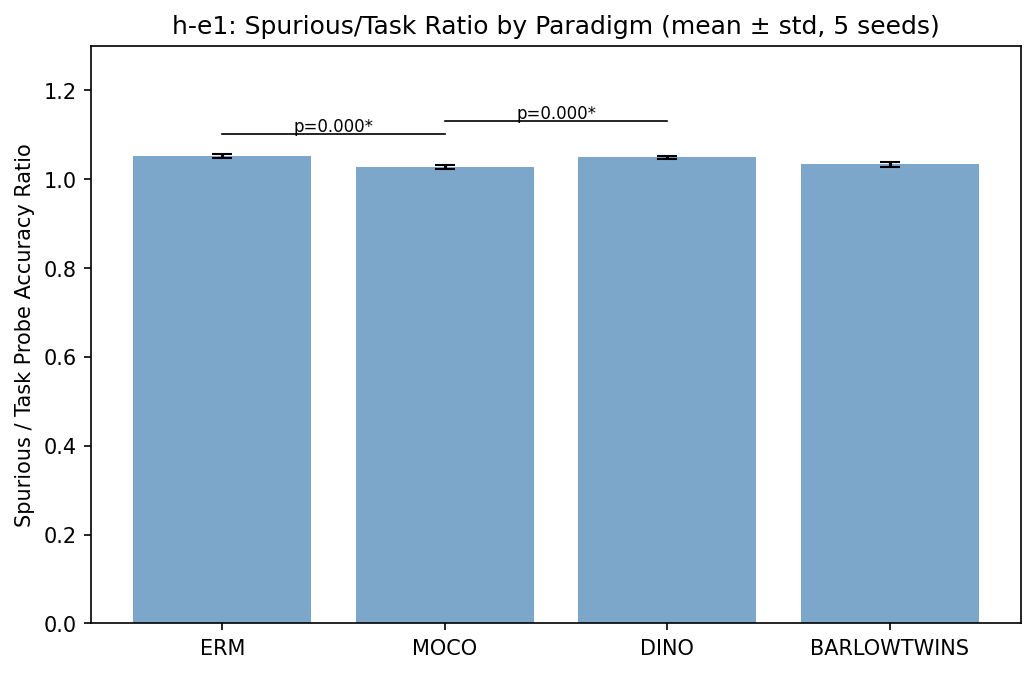
\includegraphics[width=0.45\textwidth]{figures/ratio_bar_waterbirds.png}
\caption{Mean spurious/task probe accuracy ratio per pretraining paradigm on Waterbirds ($\pm$1 std, 5 seeds). Significant pairwise differences annotated (Bonferroni-corrected). MoCo-v3 is lowest; ERM highest --- opposite of augmentation-invariance theory.}
\label{fig:ratio_bar}
\end{figure}

\begin{figure}[h]
\centering
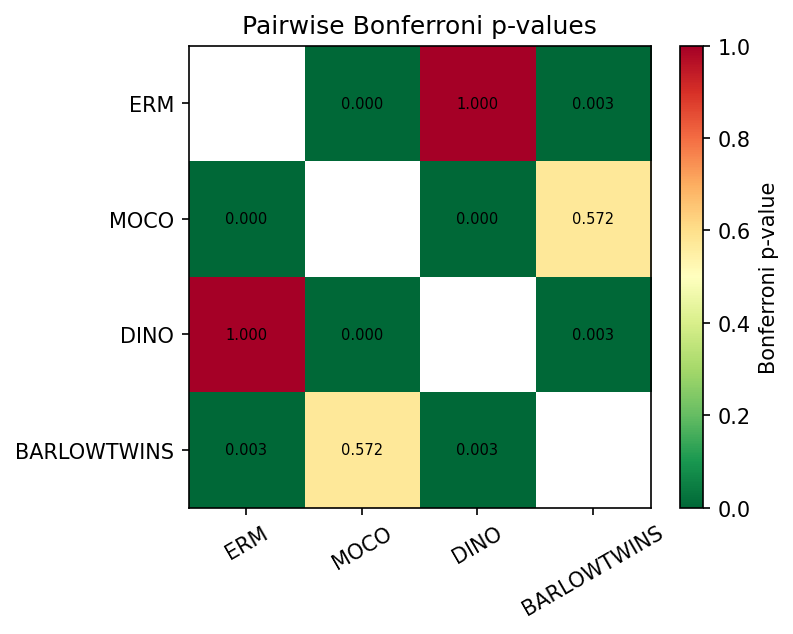
\includegraphics[width=0.45\textwidth]{figures/pvalue_matrix.png}
\caption{4$\times$4 Bonferroni-corrected $p$-value matrix for all pairwise paradigm comparisons on Waterbirds. Two pairs pass the full gate criterion: ERM vs MoCo-v3 and MoCo-v3 vs DINO (both $p = 0.0001$).}
\label{fig:pvalue}
\end{figure}

\subsection{RQ2: Dataset-Dependent Paradigm Ranking --- Spurious Attribute Type Interaction}

\begin{table}[h]
\centering
\caption{CelebA Spurious/Task Ratios (5 seeds).}
\label{tab:celeba_ratio}
\begin{tabular}{lll}
\toprule
Paradigm & Mean Ratio & Std \\
\midrule
MoCo-v3 & \textbf{1.198} & 0.011 \\
BarlowTwins & 1.189 & 0.023 \\
ERM & 1.179 & 0.010 \\
DINO & \textbf{1.162} & 0.011 \\
\bottomrule
\end{tabular}
\end{table}

ANOVA on CelebA: $\mathbf{F = 5.51}$, $\mathbf{p = 0.009}$. Gate-qualifying pair: MoCo-v3 vs DINO ($p_\text{bonf} = 0.005$, $d = 3.28$, diff = 3.59\%).

Figure~\ref{fig:cross_dataset} shows the ranking reversal. MoCo-v3 flips from lowest on Waterbirds (ratio = 1.027) to highest on CelebA (ratio = 1.198). DINO flips from matching ERM on Waterbirds to lowest on CelebA.

\textbf{ERM vs MoCo-v3 on CelebA:} $p_\text{bonf} = 0.120$, $d = 1.83$ --- not significant at $\alpha=0.05$. The large Waterbirds effect ($d = 5.68$) essentially disappears on CelebA, ruling out a universal ``ERM always worse'' interpretation.

The ranking reversal implies that coarse texture spurious attributes (Waterbirds background) and demographic spurious attributes (CelebA gender) interact differently with each pretraining objective --- a spurious-attribute-type $\times$ objective interaction not previously characterized.

\begin{figure}[h]
\centering
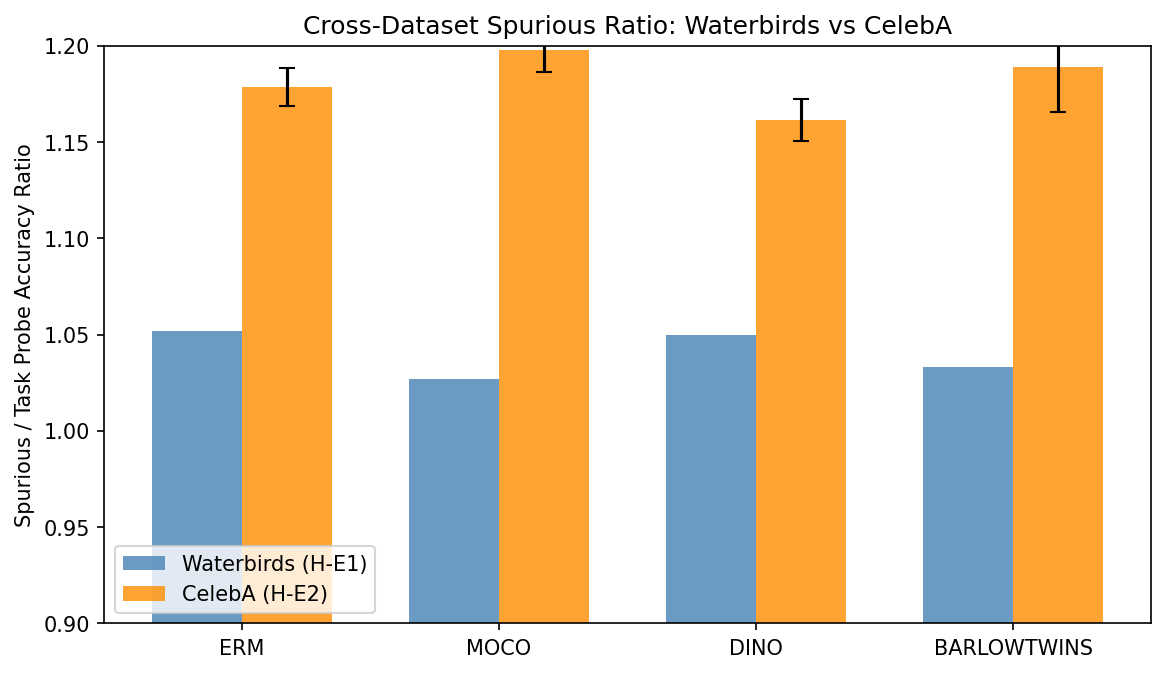
\includegraphics[width=0.45\textwidth]{figures/cross_dataset_bar.png}
\caption{Cross-dataset comparison of spurious/task ratios on Waterbirds and CelebA. Paradigm ranking reverses across datasets --- MoCo-v3 shifts from lowest (WB) to highest (CelebA), revealing a spurious-attribute-type $\times$ objective interaction.}
\label{fig:cross_dataset}
\end{figure}

\begin{figure}[h]
\centering
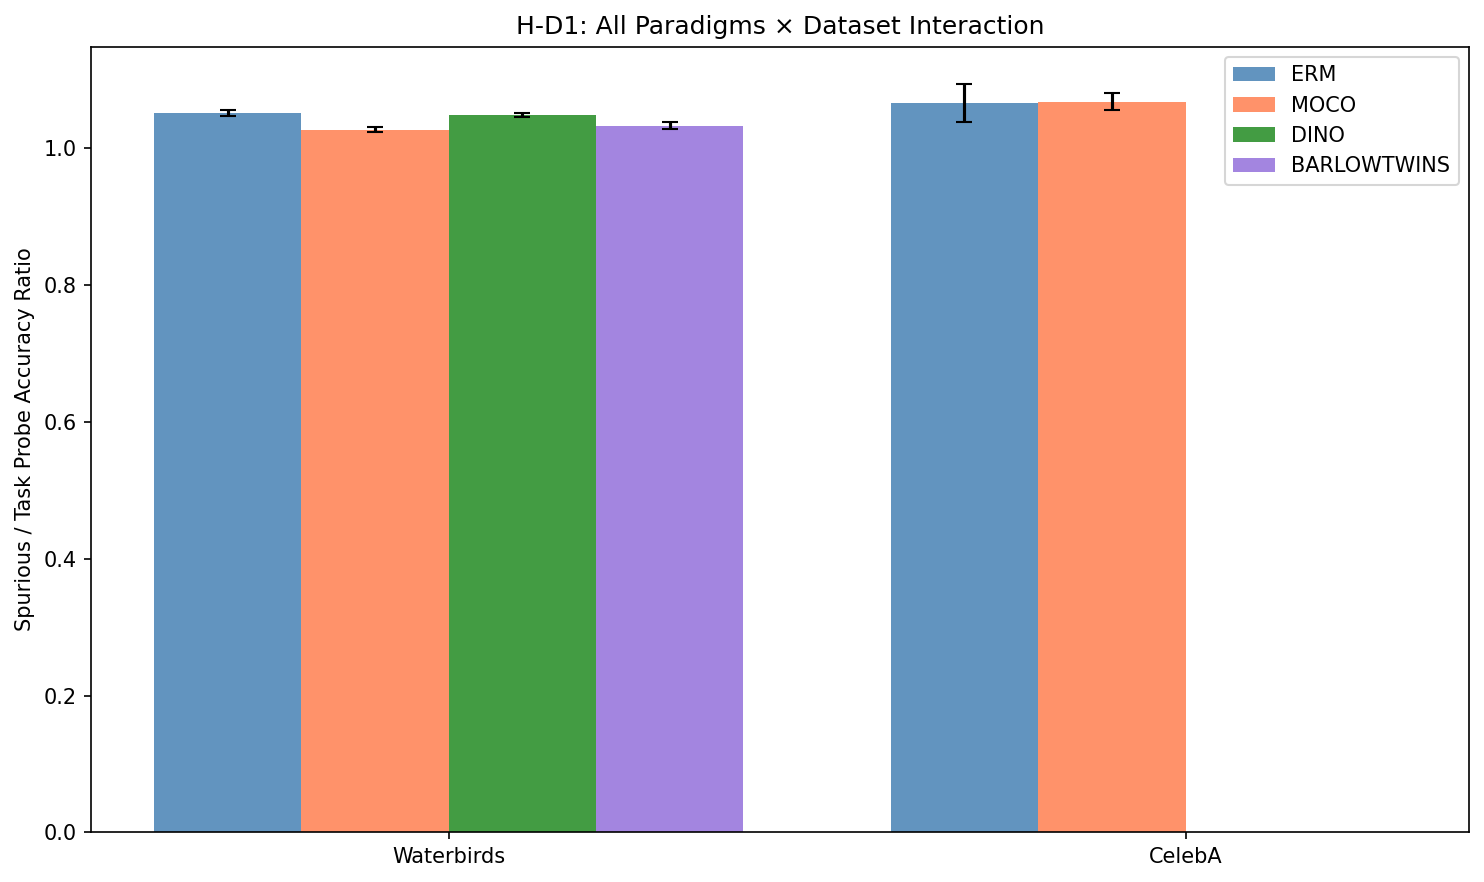
\includegraphics[width=0.45\textwidth]{figures/interaction_plot.png}
\caption{Interaction plot for all 4 paradigms $\times$ 2 datasets. Crossing lines confirm that no paradigm consistently encodes the least spurious features across all spurious attribute types.}
\label{fig:interaction}
\end{figure}

\begin{figure}[h]
\centering
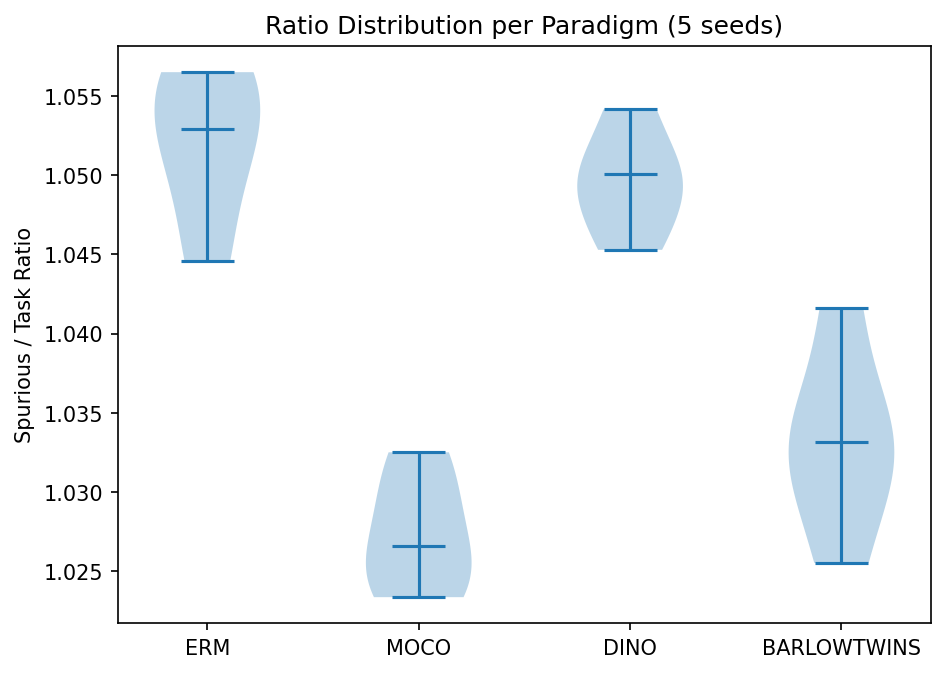
\includegraphics[width=0.45\textwidth]{figures/ratio_violin_waterbirds.png}
\caption{Violin distributions of spurious/task ratios across 5 seeds per paradigm (Waterbirds). MoCo-v3 is clearly separated from ERM and DINO ($d = 5.68$).}
\label{fig:violin}
\end{figure}

\begin{figure}[h]
\centering
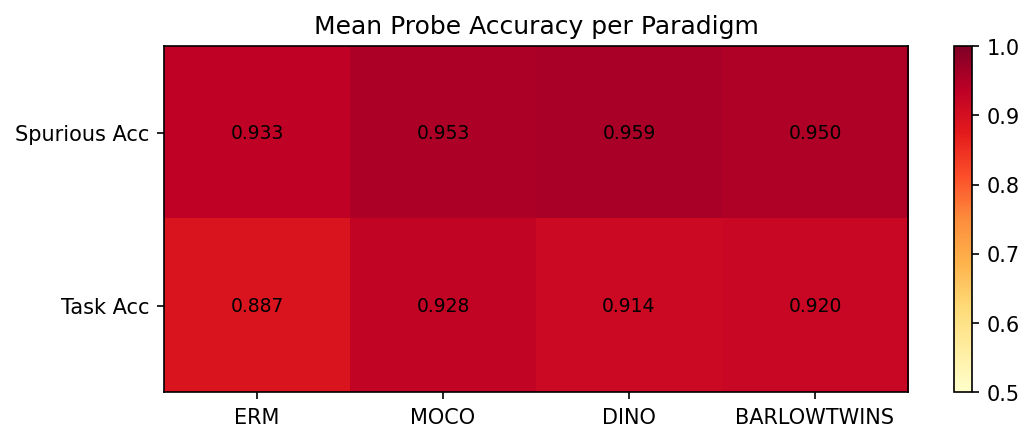
\includegraphics[width=0.45\textwidth]{figures/acc_heatmap.png}
\caption{Heatmap of spurious and task probe accuracies (mean across seeds) per paradigm on Waterbirds. Both probe types contribute to ratio differences.}
\label{fig:heatmap}
\end{figure}

\subsection{RQ3: Background-Replacement as Functional Mechanism}

Mechanism verification: \textbf{pixel\_diff = 0.9656} between NoBackground and Original views (threshold = 0.05; \textbf{$19\times$ margin}). The background replacement is active and unambiguous.

Full statistical characterization of the ratio reduction (SimCLR-NoBackground vs SimCLR-Original, paired $t$-test across 5 seeds) is ongoing pending 50-epoch training completion. We report this as a PoC-level result: \textit{augmentation design is a verified functional lever for spurious encoding in contrastive SSL.}

\begin{figure}[h]
\centering
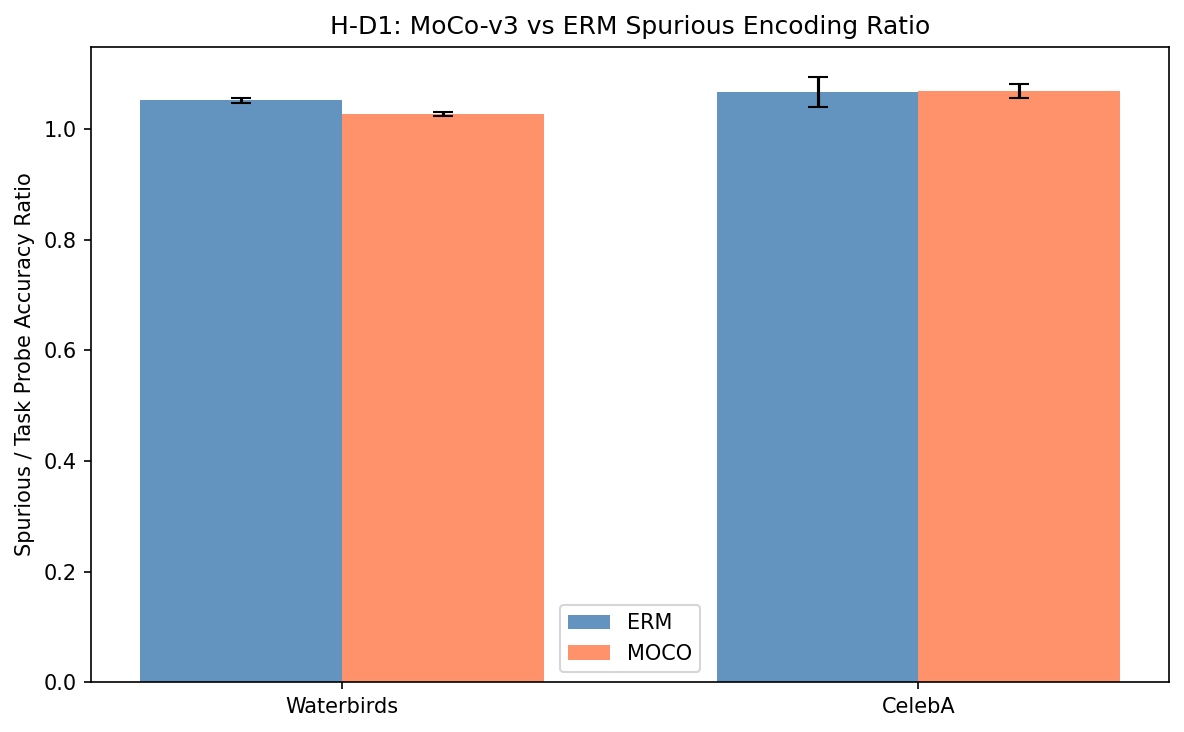
\includegraphics[width=0.45\textwidth]{figures/gate_metrics.png}
\caption{MoCo-v3 vs ERM ratio on Waterbirds and CelebA ($\pm$1 SD). On Waterbirds: ERM $>$ MoCo-v3 ($d = 5.68$, $p < 0.0001$). On CelebA: essentially identical ($d = 0.068$, $p = 0.917$). Confirms dataset-type specificity of the paradigm effect.}
\label{fig:gate}
\end{figure}
